\documentclass{standalone}
\usepackage{pgfplots}
\pgfplotsset{width=7cm,compat=1.8}

\begin{document}
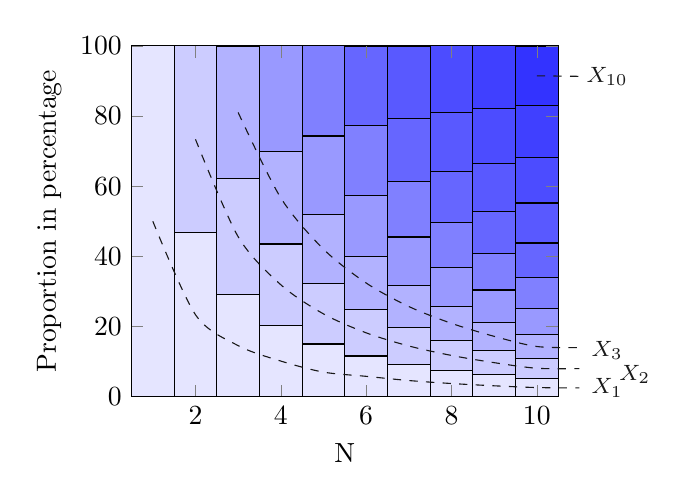
\begin{tikzpicture}
\begin{axis}[
  ybar stacked,
  bar width=1,
  axis on top,
  xmin=0.5,
  xmax=10.5,
  ymin=0,
  ymax=100,
  xlabel={N},
  ylabel={Proportion in percentage},
  after end axis/.code={
    \draw [color=black!90!white,dashed,smooth] plot coordinates{(axis cs:1,50) (axis cs:2,23.35) (axis cs:3,14.55) (axis cs:4,10.15) (axis cs:5,7.0) (axis cs:6,5.8) (axis cs:7,4.6) (axis cs:8,3.75) (axis cs:9,3.1) (axis cs:10,2.6) (axis cs:11,2.5)} node [xshift=1em,font=\footnotesize] {$X_1$};
    \draw [color=black!90!white,dashed,smooth] plot coordinates{(axis cs:2,73.35) (axis cs:3,45.6) (axis cs:4,31.9) (axis cs:5,23.6) (axis cs:6,18.2) (axis cs:7,14.45) (axis cs:8,11.75) (axis cs:9,9.7) (axis cs:10,8.1) (axis cs:11,8.0)} node [xshift=2em,yshift=-0.5ex,font=\footnotesize] {$X_2$};
    \draw [color=black!90!white,dashed,smooth] plot coordinates{(axis cs:3,81.0) (axis cs:4,56.65) (axis cs:5,42.05) (axis cs:6,32.4) (axis cs:7,25.7) (axis cs:8,20.9) (axis cs:9,17.2) (axis cs:10,14.3) (axis cs:11,14.0)} node [xshift=1em,yshift=-0.25ex,font=\footnotesize] {$X_3$};
    \draw [color=black!90!white,dashed,smooth] plot coordinates{(axis cs:10,91.45) (axis cs:11,91.3)} node [xshift=1em,font=\footnotesize] {$X_{10}$};
  }
  ]
\addplot[fill=blue!10!white] coordinates {(1,100) (2,46.7) (3,29.1) (4,20.3) (5,15.0) (6,11.6) (7,9.2)  (8,7.5)  (9,6.2)  (10,5.2)};
\addplot[fill=blue!20!white] coordinates {(1,0)   (2,53.3) (3,33.0) (4,23.2) (5,17.2) (6,13.2) (7,10.5) (8,8.5)  (9,7.0)  (10,5.8)};
\addplot[fill=blue!30!white] coordinates {(1,0)   (2,0)    (3,37.8) (4,26.3) (5,19.7) (6,15.2) (7,12.0) (8,9.8)  (9,8.0)  (10,6.6)};
\addplot[fill=blue!40!white] coordinates {(1,0)   (2,0)    (3,0)    (4,30.2) (5,22.4) (6,17.4) (7,13.8) (8,11.1) (9,9.2)  (10,7.6)};
\addplot[fill=blue!50!white] coordinates {(1,0)   (2,0)    (3,0)    (4,0)    (5,25.7) (6,19.8) (7,15.8) (8,12.8) (9,10.4) (10,8.7)};
\addplot[fill=blue!60!white] coordinates {(1,0)   (2,0)    (3,0)    (4,0)    (5,0)    (6,22.7) (7,18.0) (8,14.6) (9,12.0) (10,9.9)};
\addplot[fill=blue!65!white] coordinates {(1,0)   (2,0)    (3,0)    (4,0)    (5,0)    (6,0)    (7,20.6) (8,16.6) (9,13.7) (10,11.4)};
\addplot[fill=blue!70!white] coordinates {(1,0)   (2,0)    (3,0)    (4,0)    (5,0)    (6,0)    (7,0)    (8,19.1) (9,15.6) (10,13.0)};
\addplot[fill=blue!75!white] coordinates {(1,0)   (2,0)    (3,0)    (4,0)    (5,0)    (6,0)    (7,0)    (8,0)    (9,17.9) (10,14.8)};
\addplot[fill=blue!80!white] coordinates {(1,0)   (2,0)    (3,0)    (4,0)    (5,0)    (6,0)    (7,0)    (8,0)    (9,0)    (10,16.9)};
\addplot[fill=blue!85!white] coordinates {(1,0)   (2,0)    (3,0)    (4,0)    (5,0)    (6,0)    (7,0)    (8,0)    (9,0)    (10,0)};
\end{axis}
\end{tikzpicture}
\end{document}
1